\documentclass[10pt,twocolumn,letterpaper]{article}
% IEEE conference-style layout built from standard packages (IEEEtran.cls was not
% available offline): Times text, 0.75in margins, Roman-numbered small-caps sections.
\usepackage[margin=0.75in,columnsep=0.25in]{geometry}
\usepackage[T1]{fontenc}
\usepackage{mathptmx}
\usepackage{microtype}
\usepackage{graphicx}
\usepackage{booktabs}
\usepackage{longtable}
\usepackage{array}
\usepackage{float}
\usepackage[font=footnotesize,labelfont=bf]{caption}
\usepackage{cite}
\usepackage{url}
\usepackage[hidelinks]{hyperref}
\usepackage{titlesec}
\usepackage{balance}
\usepackage{amsmath}

% ---- Deliverable links: fill in once each link exists and has been opened to verify it.
\def\GitHubURL{https://github.com/ndunge-mbithi/summative_intro-_to_ML}
\def\DriveURL{}
\def\VideoURL{}
\newcommand{\showlink}[2]{\ifx#1\empty\textit{#2}\else\url{#1}\fi}

\renewcommand{\thesection}{\arabic{section}}
\renewcommand{\thesubsection}{\arabic{section}.\arabic{subsection}}
\titleformat{\section}{\normalfont\bfseries\centering}{\thesection.}{0.5em}{}
\titleformat{\subsection}{\normalfont\itshape}{\thesubsection.}{0.5em}{}
\titlespacing*{\section}{0pt}{1.2ex plus .5ex}{0.8ex}
\titlespacing*{\subsection}{0pt}{1ex plus .4ex}{0.4ex}
\setlength{\parskip}{0pt}
\graphicspath{{../reports/figures/}}

\title{\vspace{-1.5em}\Large Predicting Diabetes Status from Population Health Indicators Using Traditional Machine Learning and Deep Learning}
\author{Ndunge Mutheu Mbithi\\
\small BSc Software Engineering, African Leadership University}
\date{}

\begin{document}
\twocolumn[
\begin{@twocolumnfalse}
\maketitle
\vspace{-2.5em}
\begin{center}
\small
\begin{tabular}{@{}ll@{}}
\textbf{GitHub repository:} & \showlink{\GitHubURL}{GitHub repository}\\
\textbf{Google Drive folder:} & \showlink{\DriveURL}{[link pending --- folder not yet created]}\\
\textbf{Video presentation:} & \showlink{\VideoURL}{[link pending --- video not yet recorded]}\\
\end{tabular}
\end{center}
\begin{center}
\begin{minipage}{0.88\textwidth}
\small\textbf{\textit{Abstract}---}Motivated by the large share of undiagnosed diabetes in rural sub-Saharan Africa, I compare traditional machine learning and deep learning for classifying self-reported diabetes status (no diabetes, prediabetes, diabetes) from 25 population health indicators in the 2015 CDC Behavioral Risk Factor Surveillance System. The codebook-verified data comprise 441,456 records, with 440,658 usable target labels. I ran 17 tracked experiments using a leakage-safe pipeline and TensorFlow/Keras Sequential and Functional models. On a held-out test set of 66,099 respondents, tuned gradient boosting (E07) achieved macro ROC-AUC 0.8011 and macro average precision 0.4792. The selected Functional wide-and-deep network with engineered features (E17) was close (0.8004 and 0.4779), while logistic regression reached 0.7942 and 0.4690. Diabetes was moderately ranked (E07 ROC-AUC 0.843), but prediabetes remained difficult to identify (average precision about 0.036). A validation-selected $F_2$ threshold of 0.117 raised diabetes sensitivity to 0.840, at the cost of flagging 38.1\% of respondents. Error and subgroup analyses highlight self-report limitations, reverse causation and uneven sensitivity. The models are research tools, not diagnostic systems.

\smallskip
\textbf{\textit{Index Terms}---}diabetes, BRFSS, class imbalance, gradient boosting, deep learning, population health, screening.
\end{minipage}
\end{center}

\vspace{1em}
\end{@twocolumnfalse}
]

\section{Introduction}
\label{sec:intro}

Diabetes now affects roughly one adult in ten. The International Diabetes Federation estimated that 536.6 million people aged 20--79, or 10.5\% of that age group, were living with the disease in 2021, and it expects the figure to reach 783.2 million (12.2\%) by 2045~\cite{idf2022}. Worse, many people with type~2 diabetes and most with prediabetes do not know they have it, so complications build unnoticed and much effort goes into deciding who should be tested first.

This question matters to me because of the work I want to do. My mission is to revolutionise healthcare in sub-Saharan Africa through technology, creating accessible, equitable and scalable solutions for underserved rural communities, and it is in exactly those communities that the diagnosis gap is widest. The IDF reports that 24 million African adults had diabetes in 2021 and that 54\% of them were undiagnosed~\cite{idfafrica2021}. Kenya's 2015 national STEPS survey found that more than half of adults with diabetes were unaware of their condition, and measured prevalence was lower in rural areas~\cite{mohamed2018}, where fewer people are ever tested. In a rural clinic without a laboratory, a short questionnaire administered by a community health worker is about the most scalable screening tool available. Before anyone builds such a tool, though, someone has to establish how much a questionnaire can actually reveal, and what it costs in missed cases and false alarms. That is the gap this project tries to fill.

I could not do this with African data. No openly available survey from the region yet combines a large sample with richly documented predictors; the Kenyan STEPS analysis, for example, covered 4,069 adults~\cite{mohamed2018}. Instead I use the US Behavioral Risk Factor Surveillance System (BRFSS), which interviews hundreds of thousands of adults each year about chronic conditions, behaviour, access to care and demographics~\cite{cdc2015data}, and whose 2015 file is documented variable by variable in its codebook~\cite{cdc2015codebook}. I treat it as a testbed. Whatever it teaches has to be revalidated on local data before it is used anywhere in Africa. The BRFSS has also attracted a growing machine learning literature, but as Section~\ref{sec:lit} shows, much of that work simplifies the outcome to a binary label, uses a cleaned subset of the data, and reports accuracy at default thresholds, choices that make the task look easier than it really is.

My research question is therefore: \emph{How effectively can traditional machine learning and deep learning models classify diabetes status from population health indicators, and how do their predictive performance, interpretability, computational efficiency and error patterns differ?} To answer it, I kept the survey's own three categories of no diabetes, prediabetes and diabetes, built a leakage-safe pipeline, and compared logistic regression, random forests and gradient boosting with Sequential and Functional TensorFlow/Keras networks across 17 tracked experiments, before examining the selected models' thresholds, errors, explanations and subgroup performance.

Going in, I expected gradient boosting to give the best discrimination, neural networks to match it without beating it, and logistic regression to trail only slightly. Benchmark studies point that way for tabular data~\cite{grinsztajn2022,shwartzziv2022}, clinical reviews find little advantage for complex models~\cite{christodoulou2019}, and most survey answers are simple yes/no or ordered categories whose effects are likely to be additive. I also expected prediabetes to be very hard to separate from its neighbours. Throughout, I keep in mind that the labels are self-reported answers to the question of whether a doctor ever said the person had diabetes. They are not laboratory results, and none of the models here is a diagnostic tool.

\section{Literature Review}
\label{sec:lit}

\subsection{Classifying diabetes from survey data}
The study closest to mine is by Xie \emph{et al.}~\cite{xie2019}, who built type~2 diabetes risk models from the 2014 BRFSS. Their pipeline narrowed the data considerably: of 464,644 respondents, 138,146 remained after preprocessing, the outcome was restricted to non-pregnant adults over 30, and people with prediabetes were left out altogether. They compared eight classifiers on a two-thirds/one-third holdout and applied SMOTE only to the training portion, which is the correct way to resample. Discrimination was modest and tightly bunched, with AUCs between 0.718 and 0.795. The neural network scored best on AUC and accuracy yet caught only 37.8\% of cases, so the authors recommended the decision tree for screening because it found more of them. The paper taught me to judge screening models by sensitivity, and showed how much a filtered binary outcome can flatter results. One reported ``risk factor'' also stayed with me: a recent check-up was linked to \emph{higher} risk, almost certainly because people with diabetes see doctors more often. Survey predictors can reflect a diagnosis as much as anticipate it.

Most recent work uses a cleaned derivative of the 2015 BRFSS with 253,680 rows and 21 predictors, distributed through Kaggle and the UCI repository. Majcherek \emph{et al.}~\cite{majcherek2025} compared 18 algorithms on it and reported that an Extra Trees model reached an AUC of 0.99 and accuracy above 90\%, with BMI, age, general health and income as leading SHAP features. Zafar \emph{et al.}~\cite{zafar2025} applied ADASYN oversampling to the same data and proposed a hybrid deep architecture explained with LIME and SHAP. These results are hard to reconcile with the audit by Chowdhury \emph{et al.}~\cite{chowdhury2026}, which found AUROCs of only 0.818 to 0.830 across four learners, with gradient boosting already within 0.0003 of the estimated ceiling for what the survey variables can support. An AUC of 0.99 on data with such a ceiling suggests that something in the evaluation, perhaps oversampling or duplicate rows crossing the train--test boundary, deserves a closer look. I cannot tell the cause from the published papers, so I treat those figures as reported claims rather than benchmarks. The derivative dataset also makes two choices I wanted to avoid. Its binary version counts prediabetes as diabetes, which changes the meaning of the outcome, and it drops every respondent with a missing answer, even though people who refuse questions or stop interviews early are not a random subset.

\subsection{Simple models, complex models and tabular data}
Whether flexible models beat simple ones is an old question in clinical prediction, and the evidence is sobering. Christodoulou \emph{et al.}~\cite{christodoulou2019} reviewed 71 studies containing 282 comparisons and found no difference in discrimination between logistic regression and machine learning among comparisons at low risk of bias (difference in logit AUC 0.00, 95\% CI $-0.18$ to 0.18). The apparent advantages of machine learning were concentrated in the studies with weaker designs. Kopitar \emph{et al.}~\cite{kopitar2020} similarly found no clinically relevant gain from tree ensembles over regression for early type~2 diabetes detection.

The machine learning benchmarks tell a compatible story about neural networks. Grinsztajn \emph{et al.}~\cite{grinsztajn2022} tested deep architectures against tree ensembles on 45 datasets and found that trees remained state of the art on medium-sized tabular data. They traced the gap to inductive biases: trees cope well with uninformative features, respect the orientation of the feature axes and fit irregular functions easily. Shwartz-Ziv and Armon~\cite{shwartzziv2022} found that XGBoost beat recently proposed deep tabular models on most of the very datasets those models had been introduced with, and needed less tuning to do so. Whether this holds for health surveys, where nearly every predictor is binary or ordinal, is something I test directly. The ensembles I compare descend from Friedman's gradient boosting machine~\cite{friedman2001} and Breiman's random forests~\cite{breiman2001}, and my Functional API network adapts the wide-and-deep design of Cheng \emph{et al.}~\cite{cheng2016}, which places a linear model alongside a deep one.

\subsection{Evaluating rare outcomes}
Diabetes is a minority class in any general population survey, and prediabetes is rarer still. Saito and Rehmsmeier~\cite{saito2015} showed that ROC curves can look reassuring in this situation because the false-positive rate is computed against a large pool of negatives, while precision--recall curves, whose baseline equals the prevalence, show how hard the problem really is. That argument shaped my choice of average precision as the main metric. Resampling only helps when confined to training data, and published work is not always clear about this; the TRIPOD+AI statement~\cite{collins2024} now asks authors to report such choices along with missing-data handling and outcome definitions.

\subsection{Explanations, fairness and the quality of labels}
Impurity-based importances from random forests are biased towards variables with many categories or continuous scales~\cite{strobl2007}, so I rely instead on permutation importance and SHAP~\cite{lundberg2017}, which divides each prediction among the features using Shapley values. Fairness raises a deeper problem. Obermeyer \emph{et al.}~\cite{obermeyer2019} showed that a widely used population-health algorithm under-identified Black patients because it predicted health-care cost as a stand-in for health need. A similar trap exists here. A self-reported ``ever told'' diagnosis depends on access to care, so the groups who see doctors least are also the ones most likely to be labelled wrongly. Finally, a systematic review found that BRFSS self-reports agree reasonably with other self-report surveys but less well with surveys that take physical measurements~\cite{pierannunzi2013}, which limits how far any model trained on these labels can be read clinically.

\subsection{The gap this project addresses}
Taken together, these studies leave three gaps. Machine learning work on BRFSS diabetes data usually models either a filtered binary outcome~\cite{xie2019} or the complete-case derivative with prediabetes merged into diabetes~\cite{majcherek2025,zafar2025}, so the three categories the survey actually records are rarely modelled. Evaluations tend to stop at accuracy and ROC-AUC under default thresholds, saying little about minority-class precision, threshold choice or differences between groups of people. And comparisons of traditional and deep models seldom ask whether the extra complexity buys anything over a well-tuned linear model trained on the same, leakage-safe pipeline. My project works on the raw 2015 survey, keeps prediabetes as its own class, retains respondents with missing answers, and compares both paradigms under identical preprocessing with tuned decision rules and subgroup analysis. Individual pieces of this have been done before; the contribution lies in putting them together in one transparent and reproducible comparison.

\section{Methodology}
\label{sec:method}

\subsection{Data, provenance and target}
I worked with the 2015 BRFSS combined landline and cell-phone public-use file~\cite{cdc2015data}, which holds 441,456 interviews with non-institutionalised US adults across 330 variables. My sandboxed environment could not reach the CDC website, so I took a copy of \texttt{LLCP2015.XPT} from a public research repository. Because it came from a mirror, the loader checks its record count, variable count and every target category against the official codebook~\cite{cdc2015codebook} and refuses to continue on any mismatch. Every count matched exactly (Table~\ref{tab:target}); in Colab the same loader downloads the file from the CDC.

The target, \texttt{DIABETE3}, records the answer to ``(Ever told) you have diabetes''. I grouped its answers into three classes: no diabetes (codes 3 and 2), prediabetes (code 4) and diabetes (code 1). Code 2, diabetes only during pregnancy, describes a past condition, so following CDC's convention I counted it as no diabetes. Removing the 798 ``don't know'', ``refused'' and blank answers left 440,658 respondents. I kept prediabetes separate, since merging it with diabetes would change the outcome's meaning and hide the hardest part of the problem.

\begin{table}[t]
\centering\footnotesize
\caption{\texttt{DIABETE3} categories, observed counts (identical to the codebook~\cite{cdc2015codebook}) and the 3-class target mapping.}
\label{tab:target}
\begin{tabular}{@{}clrl@{}}
\toprule
Code & Response & $n$ & Target class\\
\midrule
1 & Yes & 57,256 & Diabetes \\
2 & Yes, only during pregnancy & 3,608 & No diabetes \\
3 & No & 372,104 & No diabetes \\
4 & No, pre-/borderline diabetes & 7,690 & Prediabetes \\
7 & Don't know & 598 & removed \\
9 & Refused & 193 & removed \\
missing & Blank & 7 & removed \\
\midrule
 & Total & 441,456 & \\
\bottomrule
\end{tabular}
\end{table}


\subsection{Choosing and recoding the predictors}
I chose 25 core-questionnaire predictors linked to diabetes in the literature, covering cardiometabolic and general health, behaviour and BMI, and demographics and access to care (the full list is in the repository). I left out the optional diabetes modules, whose questions, such as insulin use, are only asked of people who already report diabetes and would leak the answer into the inputs. Race and ethnicity were kept aside for checking performance across groups and never used as model inputs.

Every recode follows the codebook and is unit-tested: ``don't know'' and ``refused'' codes became missing values rather than numbers, 88 (``no days'') became zero, and BMI was rescaled from its implied decimals. The cholesterol question needed more thought. It is only asked of people who have been tested, so 49,673 never-tested respondents appear blank, yet someone never tested has, by definition, never been told their cholesterol is high. I coded them as ``not told'' rather than discarding them.

\subsection{Preprocessing and feature engineering}
Each respondent is their own primary sampling unit, so there are no duplicate people or clusters for a random split to cut through. All preprocessing lives inside scikit-learn pipelines~\cite{pedregosa2011}, so every statistic it uses is learned from the training split alone. Missing numeric values were filled with the training median, and a binary indicator was added for each feature that had gaps, so a model could still use the fact that an answer was missing. Continuous variables were capped at their training 0.1st and 99.9th percentiles. That limits the leverage of implausible BMI values without deleting the people who reported them. Smoking status was one-hot encoded with an explicit ``missing'' category. I standardised features for logistic regression and the neural networks, whose gradient-based training is sensitive to scale, but not for the tree ensembles, which are unaffected by it.

I also engineered six features from domain knowledge: a WHO BMI category, a count of diagnosed cardiometabolic conditions, a lifestyle-risk score, combined unhealthy days capped at 30, an age-by-BMI interaction and a flag for barriers to care. The transformer that builds them learns nothing from the data, so it cannot leak information between splits.

\subsection{Splitting and evaluation design}
A stratified 70/15/15 split gave 308,460 training, 66,099 validation and 66,099 test respondents. Validation data were used to compare experiments, stop network training and tune decision rules; the test set was opened once, at the end. Searches used three-fold cross-validation on a 100,000-row training sample, a compromise forced by my two-core CPU, and I also report survey-weighted test metrics as a rough population check.

With only 1.7\% of respondents in the prediabetes class, accuracy says almost nothing, so I selected models on macro average precision, which averages the area under each class's precision--recall curve so that every class counts equally~\cite{saito2015}. Because the models almost never chose a minority class as most probable, I tuned per-class probability multipliers on validation to maximise macro-F1, the three-class equivalent of moving a threshold. For a binary screening view I chose the diabetes cut-off maximising $F_2$, which values recall twice as much as precision.

\subsection{Traditional machine learning}
The traditional models were L2-penalised multinomial logistic regression, random forests~\cite{breiman2001} and gradient boosting~\cite{friedman2001}, using scikit-learn's histogram-based implementation so that boosting on 308,460 rows was feasible on a CPU; kernel SVMs, whose cost grows faster than linearly with sample size, were left out. The boosting search drew 16 candidates over learning rate, iterations, tree size, leaf size and L2 regularisation, and the forest search 10 candidates over depth, leaf size and features per split (the ranges are listed in the notebook, Section 8.3).

\subsection{Deep learning}
The neural networks were written in TensorFlow/Keras~\cite{abadi2016} and fed through \texttt{tf.data} pipelines. The training pipeline is cached, reshuffled every epoch, batched and prefetched, while validation and test pipelines keep a fixed order. Every network ends in a three-way softmax, trained with cross-entropy and Adam for up to 60 epochs, with early stopping after six epochs without improvement, checkpointing and TensorBoard logging.

I began with a Sequential network with one 32-unit hidden layer, to see whether any non-linearity helped, then a deeper one (128, 64 and 32 units with batch normalisation, 30\% dropout and L2 decay of $10^{-4}$). From there I changed one thing at a time: learning rate ($10^{-2}$, $10^{-3}$, $10^{-4}$), batch size (512 or 4096) and softened class weights. For the Functional API I built a wide-and-deep network~\cite{cheng2016}, in which a linear branch, equivalent to logistic regression, and a regularised deep branch read the same inputs and are added before the softmax. I chose it because logistic regression had already captured most of the signal, so the deep branch only needs to learn what is left over.

\subsection{Tracking, explanation and reproducibility}
Every run was recorded with its own identifier and timestamp in a JSON log, a CSV results table and TensorBoard. All random seeds were fixed and TensorFlow's deterministic operations enabled, and running the whole notebook three times from scratch produced identical results. Explanations came from permutation importance, TreeSHAP~\cite{lundberg2017} and standardised logistic regression coefficients, and test performance was broken down by sex, age, race and ethnicity, and income. Everything ran on a two-core CPU with 8.4\,GB of RAM.

\section{Results}
\label{sec:results}

\subsection{Dataset and class distribution}
The codebook-verified BRFSS 2015 file contains 441,456 records. After removing 798 records with unusable target labels, the analysis sample contains 440,658 respondents and 25 candidate indicators. Unweighted class proportions are 85.26\% no diabetes, 1.75\% prediabetes and 12.99\% diabetes; survey-weighted diabetes prevalence is 10.5\%. Income is the most frequently missing predictor (17.97\%). Missing predictors are retained through pipeline imputation rather than complete-case deletion. The analysis is based on self-reported diagnosis, not laboratory-confirmed glycaemia.

\begin{table*}[t]
\centering\footnotesize
\caption{Experiment results on the validation set (66,099 respondents; argmax decisions). Split: stratified 70/15/15, seed 42. B = 25 base features, B+E = base + 6 engineered; CW = class weighting. Time = training seconds on 2 CPU cores. Macro AP is the selection metric; the best value is in bold. Full hyper-parameters are in Appendix~\ref{app:configs} and \texttt{reports/experiment\_log.jsonl}.}
\label{tab:experiments}
\begin{tabular}{@{}llccrcccccc@{}}
\toprule
ID & Model & Feat. & Imb. & Time (s) & Acc. & Macro F1 & Macro ROC-AUC & Macro AP & Rec.\ pre. & Rec.\ dia.\\
\midrule
E01 & LR baseline & B & -- & 5 & 0.858 & 0.397 & 0.7887 & 0.4704 & 0.00 & 0.18 \\
E02 & LR unscaled & B & -- & 26 & 0.856 & 0.389 & 0.7694 & 0.4632 & 0.00 & 0.16 \\
E03 & LR balanced & B & CW & 5 & 0.645 & 0.423 & 0.7783 & 0.4657 & 0.31 & 0.59 \\
E04 & RF baseline & B & -- & 26 & 0.860 & 0.385 & 0.7862 & 0.4780 & 0.00 & 0.14 \\
E05 & GB baseline & B & -- & 26 & 0.860 & 0.406 & 0.7918 & 0.4794 & 0.00 & 0.20 \\
E06 & GB + engineered & B+E & -- & 33 & 0.861 & 0.406 & 0.7922 & 0.4798 & 0.00 & 0.20 \\
E07 & GB tuned & B+E & -- & 84 & 0.861 & 0.406 & 0.7953 & \textbf{0.4814} & 0.00 & 0.20 \\
E08 & GB tuned, balanced & B+E & CW & 84 & 0.638 & 0.422 & 0.7771 & 0.4687 & 0.28 & 0.66 \\
E09 & RF tuned & B+E & -- & 53 & 0.860 & 0.383 & 0.7921 & 0.4782 & 0.00 & 0.14 \\
E10 & MLP 32 (Seq.) & B & -- & 28 & 0.859 & 0.398 & 0.7927 & 0.4772 & 0.00 & 0.18 \\
E11 & MLP 128-64-32 reg. (Seq.) & B & -- & 112 & 0.860 & 0.390 & 0.7956 & 0.4791 & 0.00 & 0.16 \\
E12 & E11, lr $10^{-2}$ & B & -- & 33 & 0.858 & 0.359 & 0.7893 & 0.4728 & 0.00 & 0.09 \\
E13 & E11, lr $10^{-4}$ & B & -- & 216 & 0.860 & 0.381 & 0.7958 & 0.4793 & 0.00 & 0.13 \\
E14 & E11, batch 4096 & B & -- & 130 & 0.860 & 0.381 & 0.7949 & 0.4791 & 0.00 & 0.13 \\
E15 & E11, class-weighted & B & CW & 78 & 0.834 & 0.454 & 0.7959 & 0.4785 & 0.00 & 0.50 \\
E16 & Wide-and-deep (Func.) & B & -- & 106 & 0.860 & 0.399 & 0.7956 & 0.4799 & 0.00 & 0.18 \\
E17 & E16 + engineered & B+E & -- & 104 & 0.860 & 0.396 & 0.7950 & 0.4797 & 0.00 & 0.17 \\
\bottomrule
\end{tabular}
\end{table*}


\subsection{Validation experiments}
The 17 experiment outputs from the latest notebook execution are summarised in Table~\ref{tab:experiments}. Logistic regression (E01) establishes a validation macro average precision (AP) of 0.4704. Removing scaling (E02) makes optimisation slower and less effective. Class weighting (E03) increases minority-class recall but shifts the decision boundary and lowers accuracy. The random-forest baseline (E04) reaches macro AP 0.4780; baseline gradient boosting (E05) reaches 0.4796. Adding six engineered features (E06) changes AP only slightly (0.4794), so feature engineering does not materially improve this tree-based baseline.

The randomized searches are run within the training split. For gradient boosting, the best candidate uses learning rate 0.03629, 587 iterations, 16 leaf nodes, 73 minimum samples per leaf and L2 regularisation 4.33792. The search's top candidates are tightly clustered in cross-validation AP (about 0.475), and the selected refit E07 obtains validation AP 0.4812 and macro ROC-AUC 0.7955. The tuned random forest (E09) reaches validation AP 0.4782 and macro ROC-AUC 0.7921. The latest execution records 17 experiments and selects E07 among traditional models and E17 among deep-learning models by validation macro AP.

The Sequential networks vary capacity, learning rate, batch size and class weighting. The Functional wide-and-deep network is E16; E17 adds engineered features. Their validation macro APs are 0.4798 and 0.4799 respectively, making E17 the selected deep model in this execution, though the difference is negligible. Across unweighted model families, validation macro AP remains close, while class weighting primarily changes class decisions rather than improving probability ranking. Appendix~\ref{app:configs} and the notebook's experiment log provide the experiment settings and run tracking.

\subsection{Held-out test evaluation}
The selected traditional model E07, selected deep model E17, and interpretable logistic reference E01 are evaluated on the same held-out test set of 66,099 respondents. The fresh notebook output is reproduced in Table~\ref{tab:test}. E07 has macro ROC-AUC 0.8011 and macro AP 0.4792; E17 has macro ROC-AUC 0.8004 and macro AP 0.4779; E01 has macro ROC-AUC 0.7942 and macro AP 0.4690. E07's diabetes recall is 0.5462, compared with 0.4806 for E17 and 0.5024 for E01. These values supersede the earlier report's E16 selection and test metrics.

\begin{table}[t]
\centering\footnotesize
\caption{Final held-out test results (66,099 respondents) with validation-tuned decision weights. E01 = logistic regression, E07 = tuned gradient boosting, E17 = Functional wide-and-deep + engineered network. Best value per row in bold.}
\label{tab:test}
\begin{tabular}{@{}lccc@{}}
\toprule
Metric & \textbf{E01} & \textbf{E07} & \textbf{E17}\\
\midrule
Accuracy & 0.805 & 0.796 & \textbf{0.824} \\
Balanced accuracy & 0.480 & \textbf{0.498} & 0.476 \\
Macro F1 & 0.462 & \textbf{0.469} & 0.468 \\
Macro ROC-AUC & 0.794 & \textbf{0.801} & 0.800 \\
Macro AP & 0.469 & \textbf{0.479} & 0.478 \\
Recall, prediabetes & 0.072 & \textbf{0.100} & 0.056 \\
Precision, prediabetes & 0.044 & 0.042 & \textbf{0.053} \\
Recall, diabetes & 0.502 & \textbf{0.546} & 0.481 \\
Precision, diabetes & 0.394 & 0.401 & \textbf{0.421} \\
Macro F1 (survey-weighted) & 0.478 & \textbf{0.482} & 0.481 \\
Macro ROC-AUC (survey-weighted) & 0.823 & \textbf{0.830} & 0.826 \\
Recall, diabetes (survey-weighted) & 0.469 & \textbf{0.516} & 0.458 \\
\bottomrule
\end{tabular}
\end{table}


The class-wise outputs show that prediabetes remains the weakest class: E07 recall is 0.100 and precision is 0.042, while its diabetes recall is 0.546 and precision is 0.401. Its diabetes-versus-rest ROC-AUC is 0.843 and average precision is 0.434, against a 0.130 prevalence baseline. Prediabetes average precision is approximately 0.036 against a 0.017 baseline. Macro averages therefore describe a task where the dominant no-diabetes class is much easier than either minority class.

\subsection{Screening threshold and error analysis}
For a binary screening view, the validation-selected F2 threshold in the latest execution is 0.117. On the test set it gives sensitivity 0.840, specificity 0.688, PPV 0.287, NPV 0.966 and a flag rate of 0.381. The default 0.5 threshold instead has sensitivity 0.168 and flags 0.038 of respondents. The weighted screening row reports sensitivity 0.804 and flag rate 0.289. This is a trade-off, not a universally optimal clinical operating point: the high-sensitivity threshold sends over one third of respondents for follow-up, and fewer than three in ten flags are true reported cases.

\begin{table}[t]
\centering\footnotesize
\caption{Binary screening view (diabetes vs.\ not) for tuned gradient boosting on the test set. The $F_2$ threshold was selected on validation.}
\label{tab:screening}
\begin{tabular}{@{}lcccccc@{}}
\toprule
Rule & Thr. & Sens. & Spec. & PPV & NPV & Flagged\\
\midrule
Default 0.5 & 0.500 & 0.168 & 0.982 & 0.581 & 0.888 & 0.038 \\
$F_2$-optimal & 0.112 & 0.847 & 0.680 & 0.283 & 0.967 & 0.389 \\
$F_2$-optimal, weighted & 0.112 & 0.809 & 0.764 & 0.287 & 0.971 & 0.296 \\
\bottomrule
\end{tabular}
\end{table}


The latest error-profile output shows detected diabetes cases are older (mean age 66.18) and have higher BMI (33.92) and more cardiometabolic conditions (2.28) than missed cases (age 62.42, BMI 28.83, count 1.23). Among true prediabetes respondents, 52.9\% are assigned to no diabetes, 37.1\% to diabetes and 10.0\% to prediabetes. The classifier therefore tends to place prediabetes between its adjacent classes rather than identify it as a separate group.

\subsection{Explanations and subgroup results}
Permutation importance from the latest run ranks BMI (macro-AP decrease 0.0343), self-rated general health (0.0292), age (0.0164), high blood pressure (0.0112) and high cholesterol (0.0084) highest. SHAP on transformed features instead ranks general health (mean absolute value 0.3088), cardiometabolic count (0.2495), age-by-BMI (0.2195) and check-up recency (0.1607). These rankings differ because correlated and engineered features share attribution. Logistic regression coefficients provide a complementary directional view; poorer general health, age, BMI and high blood pressure are associated with higher predicted diabetes odds. These are predictive associations, not causal effects.

\begin{table}[t]
\centering\footnotesize
\caption{Test-set diabetes detection by subgroup (tuned gradient boosting, tuned decision weights). Race/ethnicity was not a model input. All subgroups have at least 163 diabetes cases.}
\label{tab:subgroups}
\setlength{\tabcolsep}{3.5pt}
\begin{tabular}{@{}llrcccc@{}}
\toprule
Dim. & Group & $n$ & Prev. & Recall & Prec. & AUC\\
\midrule
sex & Female & 37,957 & 0.124 & 0.533 & 0.401 & 0.846 \\
sex & Male & 28,142 & 0.138 & 0.563 & 0.401 & 0.839 \\
age & 45-64 & 25,676 & 0.131 & 0.521 & 0.401 & 0.832 \\
age & 65+ & 22,944 & 0.205 & 0.600 & 0.399 & 0.768 \\
age & 18-44 & 17,479 & 0.030 & 0.227 & 0.426 & 0.877 \\
race/ethnicity & White NH & 50,483 & 0.121 & 0.540 & 0.382 & 0.840 \\
race/ethnicity & Hispanic & 5,223 & 0.145 & 0.566 & 0.472 & 0.866 \\
race/ethnicity & Black NH & 5,127 & 0.205 & 0.594 & 0.450 & 0.813 \\
race/ethnicity & Other NH & 2,946 & 0.125 & 0.472 & 0.458 & 0.869 \\
race/ethnicity & Multiracial NH & 1,241 & 0.131 & 0.571 & 0.429 & 0.871 \\
income & \$50k+ & 26,238 & 0.090 & 0.434 & 0.382 & 0.856 \\
income & \$20-50k & 18,562 & 0.152 & 0.580 & 0.405 & 0.825 \\
income & <\$20k & 9,620 & 0.199 & 0.646 & 0.426 & 0.816 \\
\bottomrule
\end{tabular}
\end{table}


The updated subgroup table shows diabetes recall of 0.533 for women and 0.563 for men. Recall is 0.227 among ages 18--44, 0.521 among ages 45--64 and 0.600 among ages 65+. By race/ethnicity, recall ranges from 0.472 for Other non-Hispanic respondents to 0.594 for Black non-Hispanic respondents; the respective AUCs are 0.869 and 0.813. The latest outputs show substantial differences by age and other strata under a common rule. These are descriptive findings; they do not establish the cause of disparities or fairness on their own.

\section{Discussion}
\label{sec:discussion}

\subsection{Traditional models and deep learning}
The latest notebook execution supports a restrained conclusion: traditional machine learning and deep learning perform similarly on these tabular survey indicators. E07 tuned gradient boosting leads the validation selection at macro AP 0.4812, while E17 Functional wide-and-deep is the best deep model at 0.4799. On test data their macro ROC-AUC values are 0.8011 and 0.8004, and macro AP values are 0.4792 and 0.4779. This is a small separation, not evidence that one paradigm dominates. Logistic regression remains a useful transparent baseline (test macro AP 0.4690), close enough to make complexity and interpretability part of the practical decision.

The experiment sequence also suggests that adding capacity is not a reliable route to improvement. The two feature-engineering comparisons move macro AP only marginally, and the deep model with engineered features improves over E16 by about 0.0002 on validation AP. The dataset's indicators encode broad health status, age and healthcare contact, so flexible networks may have little new signal to discover. The search results favour regularisation and modest tree complexity rather than ever larger models. These observations are consistent with tabular-learning literature, but they should be read as evidence about this dataset and split rather than a general rule for all health data.

\subsection{Threshold choice and screening burden}
A ranking metric does not determine how many people should be referred for follow-up. At the default threshold, the E07 classifier catches only 16.8\% of diabetes cases. Lowering the threshold to 0.117 raises sensitivity to 84.0\%, but specificity falls to 68.8\%, PPV to 28.7\%, and the flag rate rises to 38.1\%. This is a sizeable screening workload. The threshold was selected by validation F2, which values recall more than precision; it is not a medical recommendation and should not be transferred to a clinic without local evaluation, calibration and a defined follow-up capacity.

The class-weighted experiments and validation-tuned decision weights also illustrate that class recall can move substantially without a corresponding gain in threshold-free ranking. A report that emphasised accuracy alone would conceal the fact that prediabetes is rarely recognised and that a high-sensitivity diabetes rule generates many false-positive flags. The useful output for a screening workflow would be a prioritisation for confirmatory testing, not a diagnosis.

\subsection{Labels, explainability and equity}
The outcome records whether a respondent was told they had diabetes. It cannot distinguish a true negative from a person who has diabetes but has not been tested or informed. As a result, some false-positive flags may resemble plausible undiagnosed cases, while people with limited access to care can be mislabelled in the training target. The weak prediabetes performance is especially consequential because the category is both uncommon and dependent on prior testing. The current models learn the survey's diagnosis process as well as underlying health patterns.

The explanation outputs identify BMI, general health, age, hypertension and cholesterol as useful signals, but these features should not be interpreted as causes. Check-up recency and cholesterol testing partly represent contact with the health system; a diagnosis can change both behaviour and access to care. Attribution methods also distribute importance differently across raw and engineered features, so no single ranking is definitive. Excluding race from model inputs does not eliminate subgroup performance differences. The current subgroup outputs show low recall among younger adults and variation across race/ethnicity and income, which warrants careful local assessment rather than a claim that the model is fair or unfair.

\subsection{Implications for rural sub-Saharan Africa}
The project is motivated by communities where laboratory screening may be difficult to access, but BRFSS is a US telephone survey from 2015. Its predictors, diagnosis pathways, and prevalence are not a substitute for data collected in rural African settings. The results support investigating low-cost questionnaire-based triage, not deploying this model directly. Logistic regression is attractive as a transparent, lightweight baseline; however, local labels and clinical validation matter more than choosing a sophisticated architecture.

A responsible next step would collect laboratory-confirmed glycaemic measurements alongside questionnaire indicators, include communities with varied access to care, and evaluate sensitivity, calibration and referral burden by subgroup. Decision thresholds should be agreed with health workers and clinics based on the availability of confirmatory tests. Only after external and prospective validation should a model be considered for real screening support.

\subsection{Limitations and next work}
This analysis uses one cross-sectional year, self-reported labels, and a subsample for hyperparameter search. The test metrics are not a complete design-based evaluation of BRFSS's complex survey structure, and calibration was not comprehensively assessed. Results may shift across years or populations. Future work should compare the classifier with laboratory-defined outcomes, use survey-aware estimation, evaluate calibration and threshold stability, and validate on later BRFSS data and locally collected African cohorts. These steps would address the main limitations before any clinical use.

\section{Conclusion}
\label{sec:conclusion}

I compared traditional machine learning and TensorFlow/Keras models for classifying no diabetes, prediabetes and diabetes from 25 indicators in 440,658 labelled respondents from BRFSS 2015. In the latest notebook execution, tuned gradient boosting (E07) is the selected traditional model and Functional wide-and-deep with engineered features (E17) is the selected deep model. On the held-out test set, E07 reaches macro ROC-AUC 0.8011 and macro AP 0.4792; E17 reaches 0.8004 and 0.4779. Logistic regression remains close and easier to interpret. Prediabetes is poorly distinguished, while the diabetes screening threshold trades a sensitivity of 0.840 for a flag rate of 0.381.

The main lesson is that the operating threshold, outcome quality and population fit matter at least as much as model family. These self-reported US survey labels cannot identify undiagnosed diabetes reliably and the subgroup results show that a single rule does not perform equally across groups. The model is a research exercise, not a diagnostic system. Before considering a screening application in sub-Saharan Africa, I would collect laboratory-confirmed local data, assess calibration and survey-aware performance, and set referral thresholds with clinics according to their confirmatory-testing capacity.


\balance
\begin{thebibliography}{99}
\footnotesize
\bibitem{idf2022} H. Sun \emph{et al.}, ``IDF Diabetes Atlas: Global, regional and country-level diabetes prevalence estimates for 2021 and projections for 2045,'' \emph{Diabetes Res. Clin. Pract.}, vol. 183, Art. no. 109119, 2022, doi: 10.1016/j.diabres.2021.109119.

\bibitem{idfafrica2021} International Diabetes Federation Africa Region, ``24m adults are living with diabetes in Africa,'' IDF, 2021. [Online]. Available: https://idf.org/?p=948

\bibitem{mohamed2018} S. F. Mohamed \emph{et al.}, ``Prevalence and factors associated with pre-diabetes and diabetes mellitus in Kenya: Results from a national survey,'' \emph{BMC Public Health}, vol. 18, suppl. 3, Art. no. 1215, 2018, doi: 10.1186/s12889-018-6053-x.

\bibitem{cdc2015data} Centers for Disease Control and Prevention, ``2015 BRFSS survey data and documentation,'' Behavioral Risk Factor Surveillance System, Aug. 2016. [Online]. Available: https://www.cdc.gov/brfss/annual\_data/annual\_2015.html

\bibitem{cdc2015codebook} Centers for Disease Control and Prevention, ``Behavioral Risk Factor Surveillance System 2015 codebook report: Land-line and cell-phone data,'' Aug. 23, 2016. [Online]. Available: https://www.cdc.gov/brfss/annual\_data/2015/pdf/codebook15\_llcp.pdf

\bibitem{grinsztajn2022} L. Grinsztajn, E. Oyallon, and G. Varoquaux, ``Why do tree-based models still outperform deep learning on typical tabular data?'' in \emph{Adv. Neural Inf. Process. Syst. (NeurIPS), Datasets and Benchmarks Track}, 2022. [Online]. Available: https://arxiv.org/abs/2207.08815

\bibitem{shwartzziv2022} R. Shwartz-Ziv and A. Armon, ``Tabular data: Deep learning is not all you need,'' \emph{Inf. Fusion}, vol. 81, pp. 84--90, 2022, doi: 10.1016/j.inffus.2021.11.011.

\bibitem{christodoulou2019} E. Christodoulou, J. Ma, G. S. Collins, E. W. Steyerberg, J. Y. Verbakel, and B. Van Calster, ``A systematic review shows no performance benefit of machine learning over logistic regression for clinical prediction models,'' \emph{J. Clin. Epidemiol.}, vol. 110, pp. 12--22, 2019, doi: 10.1016/j.jclinepi.2019.02.004.

\bibitem{xie2019} Z. Xie, O. Nikolayeva, J. Luo, and D. Li, ``Building risk prediction models for type 2 diabetes using machine learning techniques,'' \emph{Prev. Chronic Dis.}, vol. 16, Art. no. 190109, 2019, doi: 10.5888/pcd16.190109.

\bibitem{majcherek2025} D. Majcherek, A. Ciesielski, and P. Sobczak, ``AI-driven analysis of diabetes risk determinants in U.S. adults: Exploring disease prevalence and health factors,'' \emph{PLOS ONE}, vol. 20, no. 9, Art. no. e0328655, 2025, doi: 10.1371/journal.pone.0328655.

\bibitem{zafar2025} M. M. Zafar, Z. A. Khan, N. Javaid, M. Aslam, and N. Alrajeh, ``From data to diagnosis: A novel deep learning model for early and accurate diabetes prediction,'' \emph{Healthcare}, vol. 13, no. 17, Art. no. 2138, 2025, doi: 10.3390/healthcare13172138.

\bibitem{chowdhury2026} S. S. Chowdhury, N. Jahan, S. Mukhopadhyay, S. Fang, and V. R. Ramakrishnan, ``The ceiling is in the channel: Auditing learner gaps and measurement frontiers in clinical prediction,'' arXiv:2609.01909, Sep. 2026 (preprint).

\bibitem{kopitar2020} L. Kopitar, P. Kocbek, L. Cilar, A. Sheikh, and G. \v{S}tiglic, ``Early detection of type 2 diabetes mellitus using machine learning-based prediction models,'' \emph{Sci. Rep.}, vol. 10, Art. no. 11981, 2020, doi: 10.1038/s41598-020-68771-z.

\bibitem{friedman2001} J. H. Friedman, ``Greedy function approximation: A gradient boosting machine,'' \emph{Ann. Statist.}, vol. 29, no. 5, pp. 1189--1232, 2001, doi: 10.1214/aos/1013203451.

\bibitem{breiman2001} L. Breiman, ``Random forests,'' \emph{Mach. Learn.}, vol. 45, no. 1, pp. 5--32, 2001, doi: 10.1023/A:1010933404324.

\bibitem{cheng2016} H.-T. Cheng \emph{et al.}, ``Wide \& deep learning for recommender systems,'' in \emph{Proc. 1st Workshop Deep Learn. Recommender Syst. (DLRS)}, 2016, pp. 7--10, doi: 10.1145/2988450.2988454.

\bibitem{saito2015} T. Saito and M. Rehmsmeier, ``The precision-recall plot is more informative than the ROC plot when evaluating binary classifiers on imbalanced datasets,'' \emph{PLOS ONE}, vol. 10, no. 3, Art. no. e0118432, 2015, doi: 10.1371/journal.pone.0118432.

\bibitem{collins2024} G. S. Collins \emph{et al.}, ``TRIPOD+AI statement: Updated guidance for reporting clinical prediction models that use regression or machine learning methods,'' \emph{BMJ}, vol. 385, Art. no. e078378, 2024, doi: 10.1136/bmj-2023-078378.

\bibitem{strobl2007} C. Strobl, A.-L. Boulesteix, A. Zeileis, and T. Hothorn, ``Bias in random forest variable importance measures: Illustrations, sources and a solution,'' \emph{BMC Bioinformatics}, vol. 8, Art. no. 25, 2007, doi: 10.1186/1471-2105-8-25.

\bibitem{lundberg2017} S. M. Lundberg and S.-I. Lee, ``A unified approach to interpreting model predictions,'' in \emph{Adv. Neural Inf. Process. Syst. 30 (NIPS)}, 2017. [Online]. Available: https://papers.nips.cc/paper/7062-a-unified-approach-to-interpreting-model-predictions

\bibitem{obermeyer2019} Z. Obermeyer, B. Powers, C. Vogeli, and S. Mullainathan, ``Dissecting racial bias in an algorithm used to manage the health of populations,'' \emph{Science}, vol. 366, no. 6464, pp. 447--453, 2019, doi: 10.1126/science.aax2342.

\bibitem{pierannunzi2013} C. Pierannunzi, S. S. Hu, and L. Balluz, ``A systematic review of publications assessing reliability and validity of the Behavioral Risk Factor Surveillance System (BRFSS), 2004--2011,'' \emph{BMC Med. Res. Methodol.}, vol. 13, Art. no. 49, 2013, doi: 10.1186/1471-2288-13-49.

\bibitem{pedregosa2011} F. Pedregosa \emph{et al.}, ``Scikit-learn: Machine learning in Python,'' \emph{J. Mach. Learn. Res.}, vol. 12, pp. 2825--2830, 2011.

\bibitem{abadi2016} M. Abadi \emph{et al.}, ``TensorFlow: A system for large-scale machine learning,'' in \emph{Proc. 12th USENIX Symp. Operating Syst. Design Implementation (OSDI)}, 2016, pp. 265--283.

\end{thebibliography}

\onecolumn
\appendix
\section{Experiment configurations}
\label{app:configs}
Every row below corresponds to a run in \texttt{reports/experiment\_log.jsonl} and a TensorBoard directory \texttt{logs/tensorboard/<run ID>}. All runs used the same stratified 70/15/15 split (seed 42). Traditional models used median imputation with missing-value indicators, 0.1/99.9\% winsorising of continuous variables and one-hot encoded smoking status; logistic regression (except E02) and all networks were also standardised. Run IDs are from the final reported execution.

\begin{footnotesize}
\begin{longtable}{@{}p{0.04\linewidth}p{0.17\linewidth}p{0.41\linewidth}p{0.32\linewidth}@{}}
\toprule
ID & Run ID & Hyper-parameters & Observation (after reading the results)\\
\midrule
\endhead
E01 & \texttt{E01\_20261018T073349Z} & C=1.0, penalty=l2, solver=lbfgs, max\_iter=1000 & Reference model: converges in 36 iterations; 0.86 accuracy hides 0 prediabetes and 0.18 diabetes recall under argmax. \\
E02 & \texttt{E02\_20261018T073416Z} & C=1.0, penalty=l2, solver=lbfgs, max\_iter=200, scaling=False & Without scaling, L-BFGS hits its 200-iteration cap (convergence warning), runs ~5x slower and is worse than E01 on every metric. \\
E03 & \texttt{E03\_20261018T073421Z} & C=1.0, penalty=l2, solver=lbfgs, max\_iter=1000 & Balanced weights vs E01: diabetes recall 0.18->0.59, prediabetes 0->0.31, but accuracy 0.645 and macro AP drops slightly; threshold moved, ranking not improved. \\
E04 & \texttt{E04\_20261018T073449Z} & n\_estimators=150, max\_depth=None, min\_samples\_leaf=5, max\_features=sqrt & Fully grown trees (mean depth ~39, ~13k leaves): macro AP above E01 but ROC-AUC below it, the signature of a high-variance learner. \\
E05 & \texttt{E05\_20261018T073517Z} & learning\_rate=0.1, max\_iter=200, max\_leaf\_nodes=31, min\_samples\_leaf=20 & Boosting improves both macro AP and ROC-AUC over the forest: sequential bias reduction beats averaging deep trees here. \\
E06 & \texttt{E06\_20261018T073551Z} & learning\_rate=0.1, max\_iter=200, max\_leaf\_nodes=31, min\_samples\_leaf=20 & Engineered features add only +0.0004 macro AP to E05; trees already form interactions such as age x BMI by splitting. \\
E07 & \texttt{E07\_20261018T075447Z} & l2\_regularization=4.33792, learning\_rate=0.03629, max\_iter=587, max\_leaf\_nodes=16, min\_samples\_leaf=73 & Search picks the most regularised candidate (lr 0.036, 16 leaves, L2 4.34; train-fold 0.625 vs CV 0.475): best macro AP of all runs. \\
E08 & \texttt{E08\_20261018T075614Z} & l2\_regularization=4.33792, learning\_rate=0.03629, max\_iter=587, max\_leaf\_nodes=16, min\_samples\_leaf=73 & Balanced weights on E07 repeat the E03 pattern: diabetes recall 0.66, prediabetes 0.28, macro AP lower. \\
E09 & \texttt{E09\_20261018T080006Z} & max\_depth=14, max\_features=0.1572, min\_samples\_leaf=6, n\_estimators=300 & Shallower forest (depth 14, ~16\% features per split) raises ROC-AUC 0.786->0.792 at unchanged macro AP: regularisation smooths mid-risk ranking. \\
E10 & \texttt{E10\_20261018T080040Z} & layers=32, activation=relu, learning\_rate=0.001, dropout=0, l2=0, batch\_size=512, epochs\_run=15, best\_epoch=9, params=1763, optimizer=Adam, early\_stopping=val\_loss, patience 6 & 32-unit MLP early-stops at epoch 9 with a negligible train/val gap; beats LR slightly but trails boosting. \\
E11 & \texttt{E11\_20261018T080233Z} & layers=128-64-32, batch\_norm=True, dropout=0.3, l2=0.0001, learning\_rate=0.001, batch\_size=512, epochs\_run=29, best\_epoch=23, params=17987, optimizer=Adam, early\_stopping=val\_loss, patience 6 & Deeper MLP with BN/dropout/L2: small gain over E10; training loss above validation loss because regularisation is active only in training. \\
E12 & \texttt{E12\_20261018T080307Z} & layers=128-64-32, batch\_norm=True, dropout=0.3, l2=0.0001, learning\_rate=0.01, batch\_size=512, epochs\_run=8, best\_epoch=2, params=17987, optimizer=Adam, early\_stopping=val\_loss, patience 6 & lr 1e-2 is unstable (best epoch 2, oscillating validation loss) and loses macro AP versus E11. \\
E13 & \texttt{E13\_20261018T080645Z} & layers=128-64-32, batch\_norm=True, dropout=0.3, l2=0.0001, learning\_rate=0.0001, batch\_size=512, epochs\_run=60, best\_epoch=60, params=17987, optimizer=Adam, early\_stopping=val\_loss, patience 6 & lr 1e-4 is still improving at the 60-epoch cap and takes ~2x E11's time for the same macro AP: too slow for the budget. \\
E14 & \texttt{E14\_20261018T080856Z} & layers=128-64-32, batch\_norm=True, dropout=0.3, l2=0.0001, learning\_rate=0.001, batch\_size=4096, epochs\_run=60, best\_epoch=58, params=17987, optimizer=Adam, early\_stopping=val\_loss, patience 6 & Batch 4096 needs 58 of 60 epochs to match E11: fewer updates per epoch, no quality gain. \\
E15 & \texttt{E15\_20261018T081015Z} & layers=128-64-32, batch\_norm=True, dropout=0.3, l2=0.0001, learning\_rate=0.001, batch\_size=512, epochs\_run=19, best\_epoch=13, params=17987, optimizer=Adam, early\_stopping=val\_loss, patience 6 & Softened class weights raise diabetes recall 0.16->0.50 and macro-F1 to 0.454 with macro AP unchanged; prediabetes still never predicted. \\
E16 & \texttt{E16\_20261018T081202Z} & architecture=wide (linear) + deep 128-64, logits summed, dropout=0.3, l2=0.0001, learning\_rate=0.001, batch\_size=512, epochs\_run=29, best\_epoch=23, params=16031, optimizer=Adam, early\_stopping=val\_loss, patience 6 & Wide-and-deep is the best deep model: the linear wide path keeps the additive signal, the deep path adds little on top. \\
E17 & \texttt{E17\_20261018T081347Z} & architecture=wide (linear) + deep 128-64, logits summed, dropout=0.3, l2=0.0001, learning\_rate=0.001, batch\_size=512, epochs\_run=29, best\_epoch=23, params=17603, optimizer=Adam, early\_stopping=val\_loss, patience 6 & Engineered features give no gain on E16, consistent with E06. \\
\bottomrule
\end{longtable}
\end{footnotesize}


\section{Supplementary figures}

\begin{figure}[H]
\centering
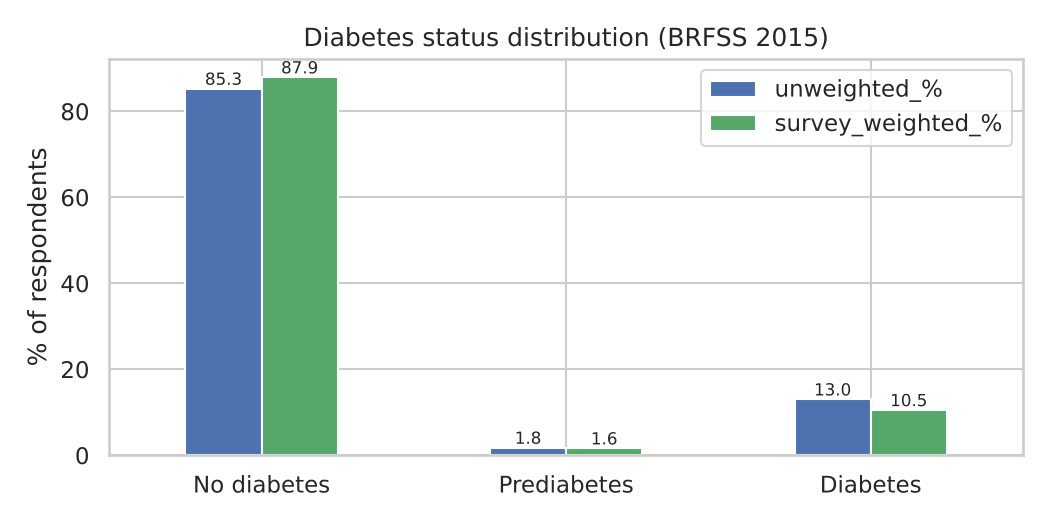
\includegraphics[width=0.48\linewidth]{fig01_target_distribution.png}\hfill
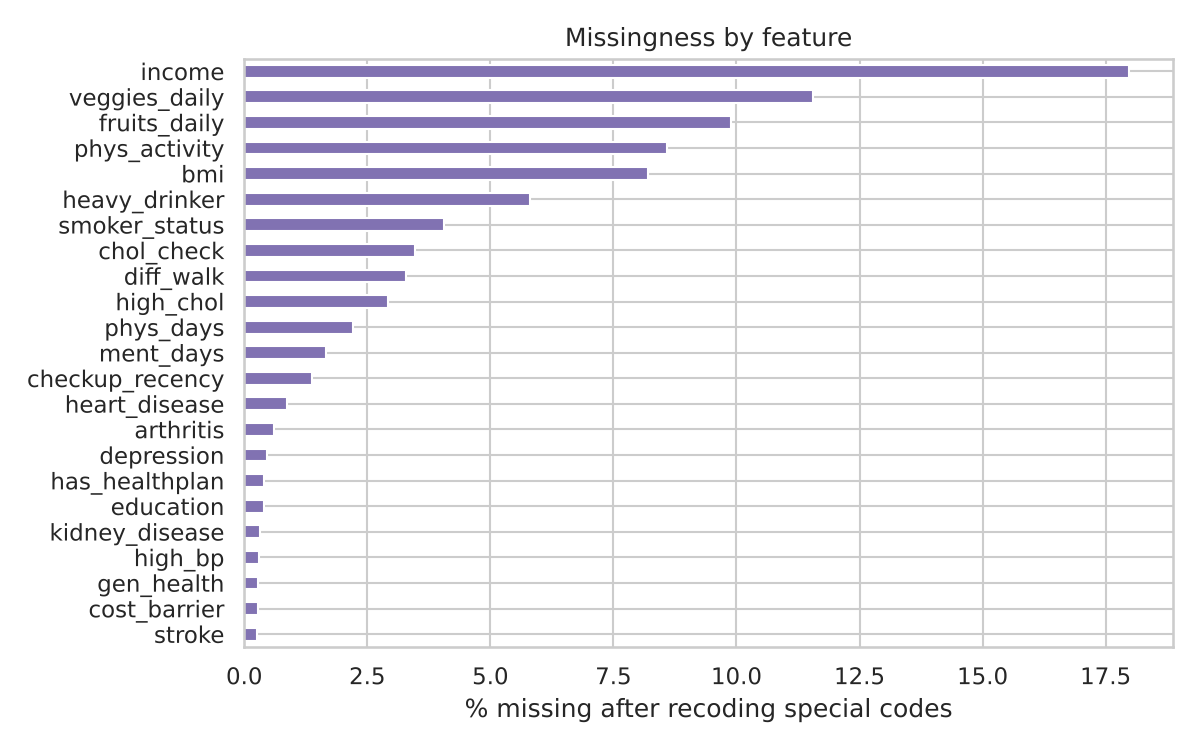
\includegraphics[width=0.48\linewidth]{fig02_missingness.png}
\caption{Left: class distribution, unweighted and survey-weighted. Right: percentage of missing values per feature after recoding special codes.}
\end{figure}

\begin{figure}[H]
\centering
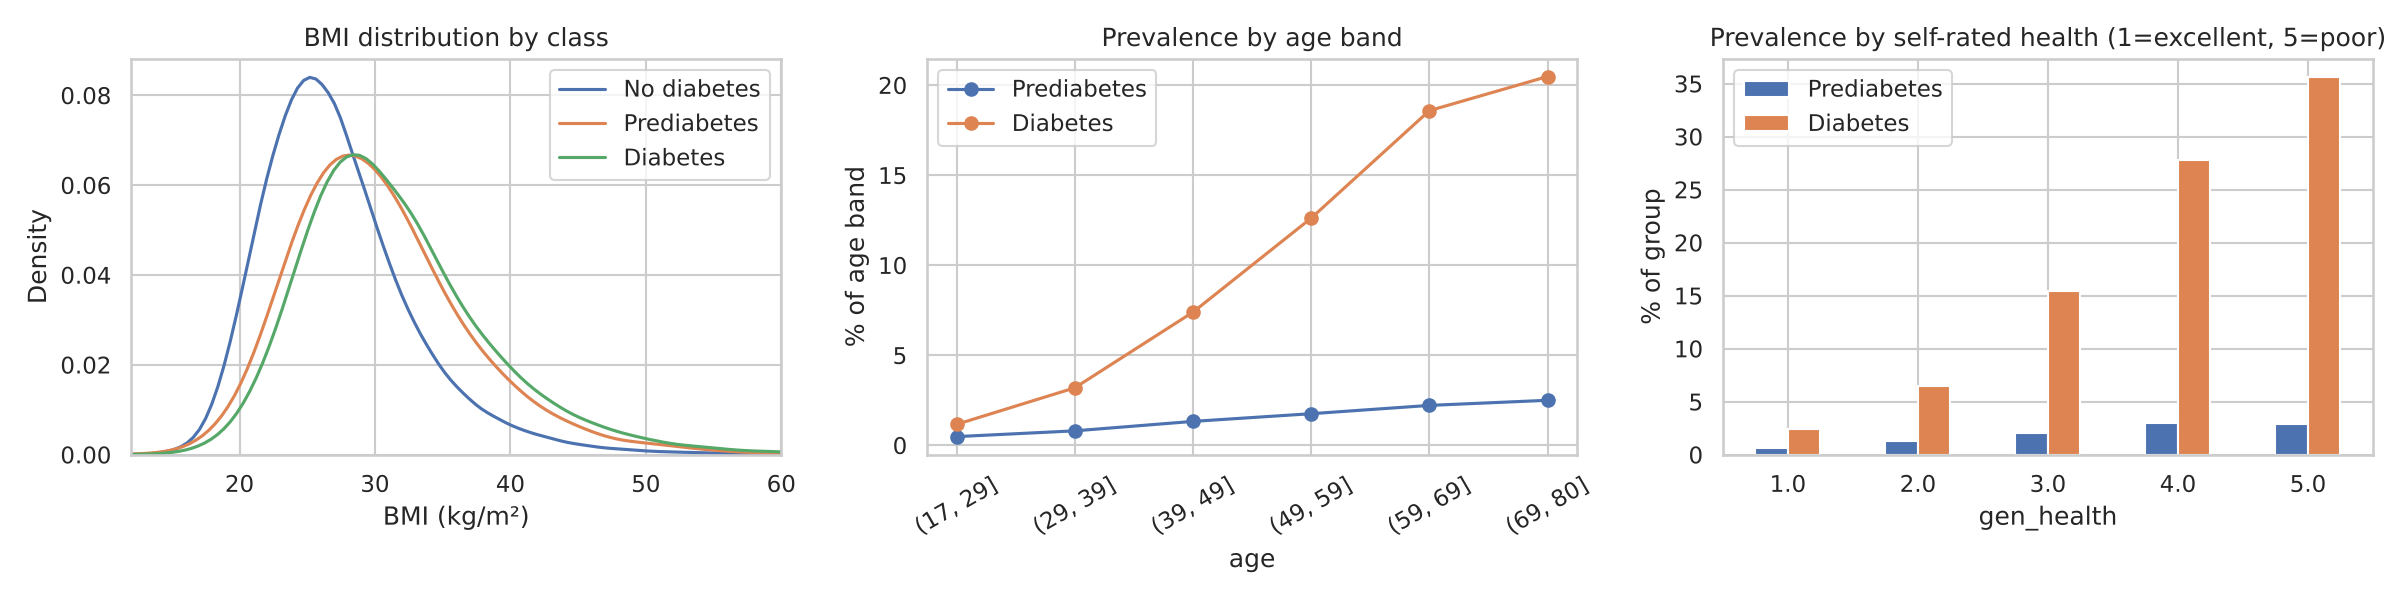
\includegraphics[width=\linewidth]{fig03_distributions.png}
\caption{BMI distribution by class, prevalence by age band, and prevalence by self-rated general health.}
\end{figure}

\begin{figure}[H]
\centering
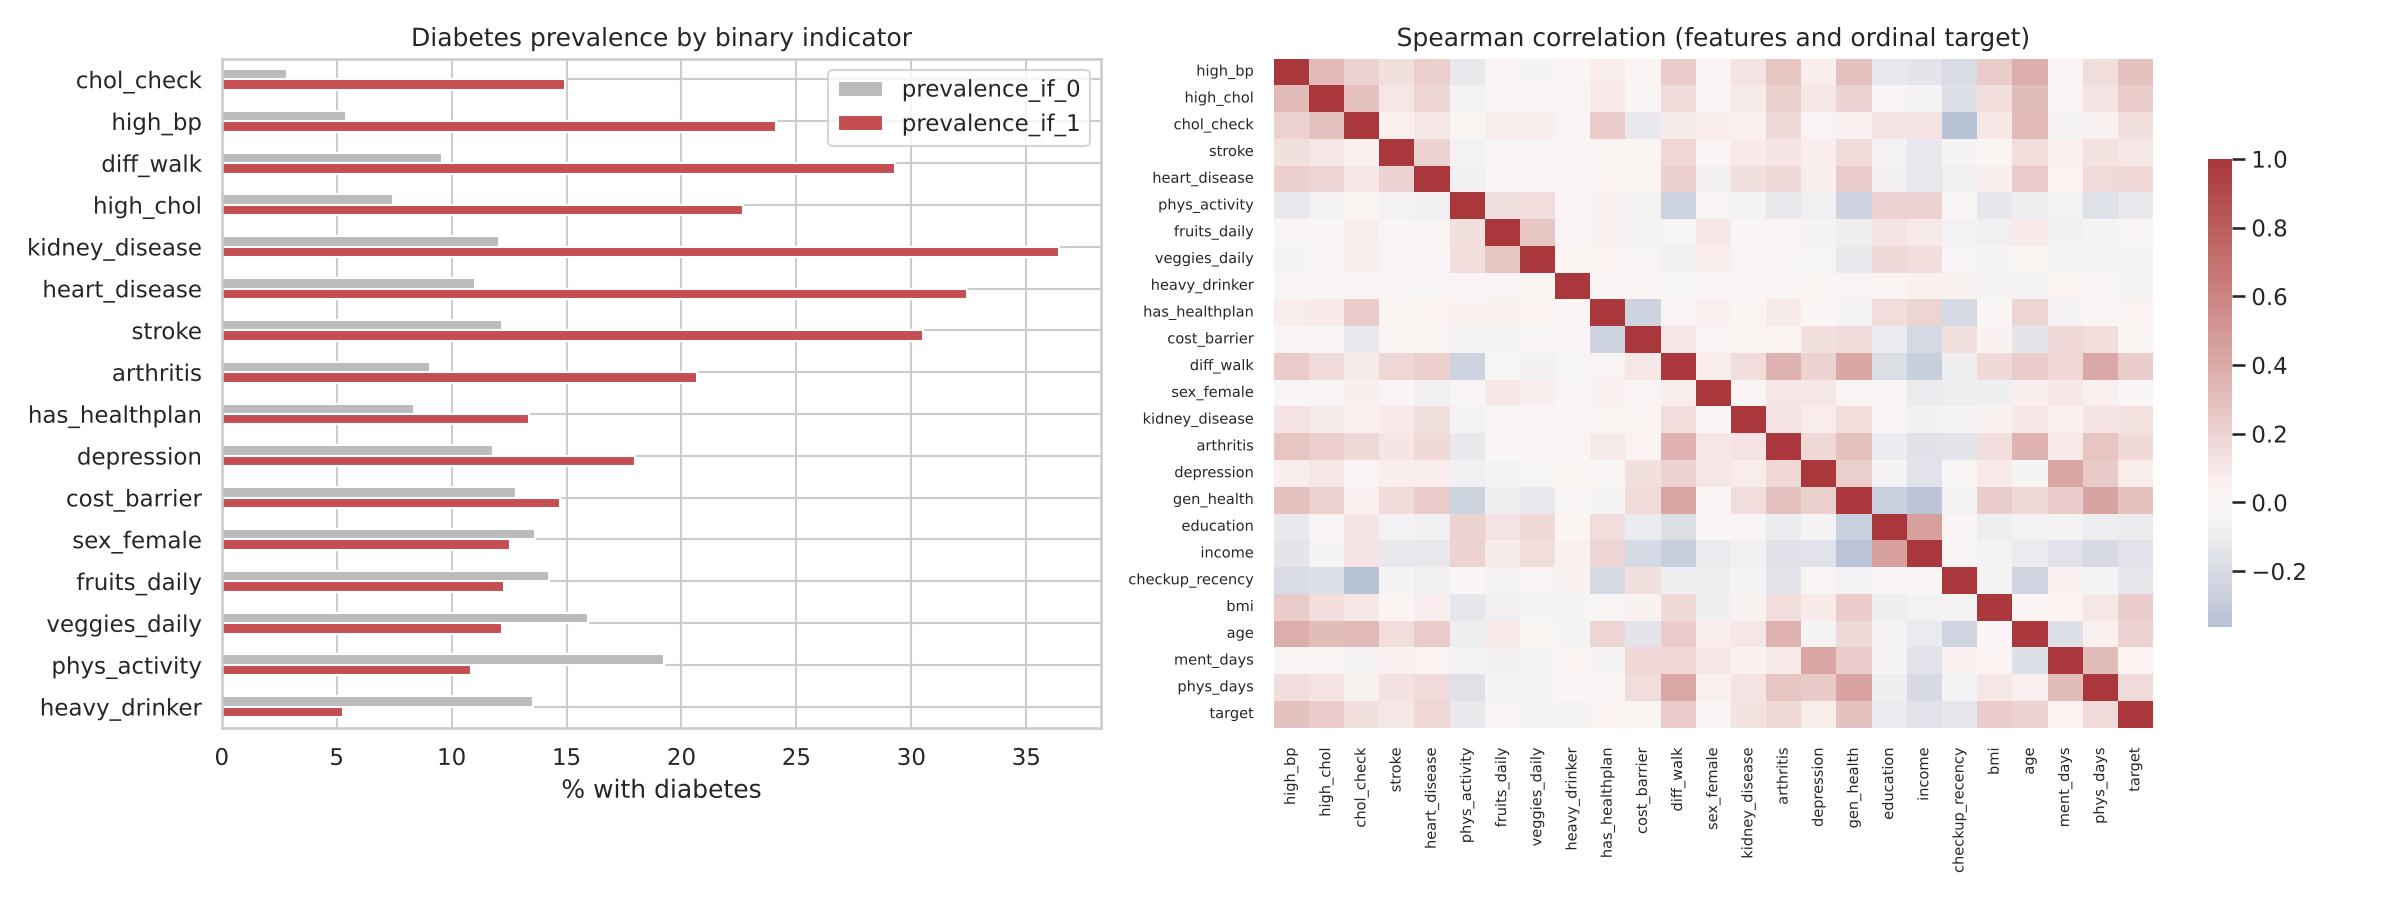
\includegraphics[width=\linewidth]{fig04_associations.png}
\caption{Diabetes prevalence by binary indicator (left) and Spearman correlations among features and the ordinal target (right).}
\end{figure}

\begin{figure}[H]
\centering
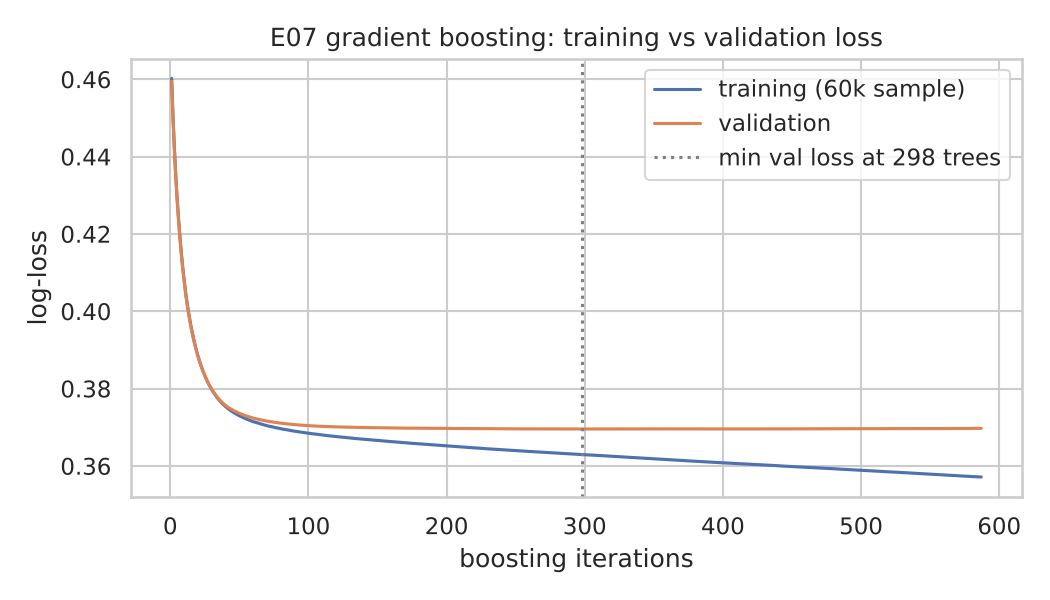
\includegraphics[width=0.48\linewidth]{fig06_boosting_learning_curve.png}\hfill
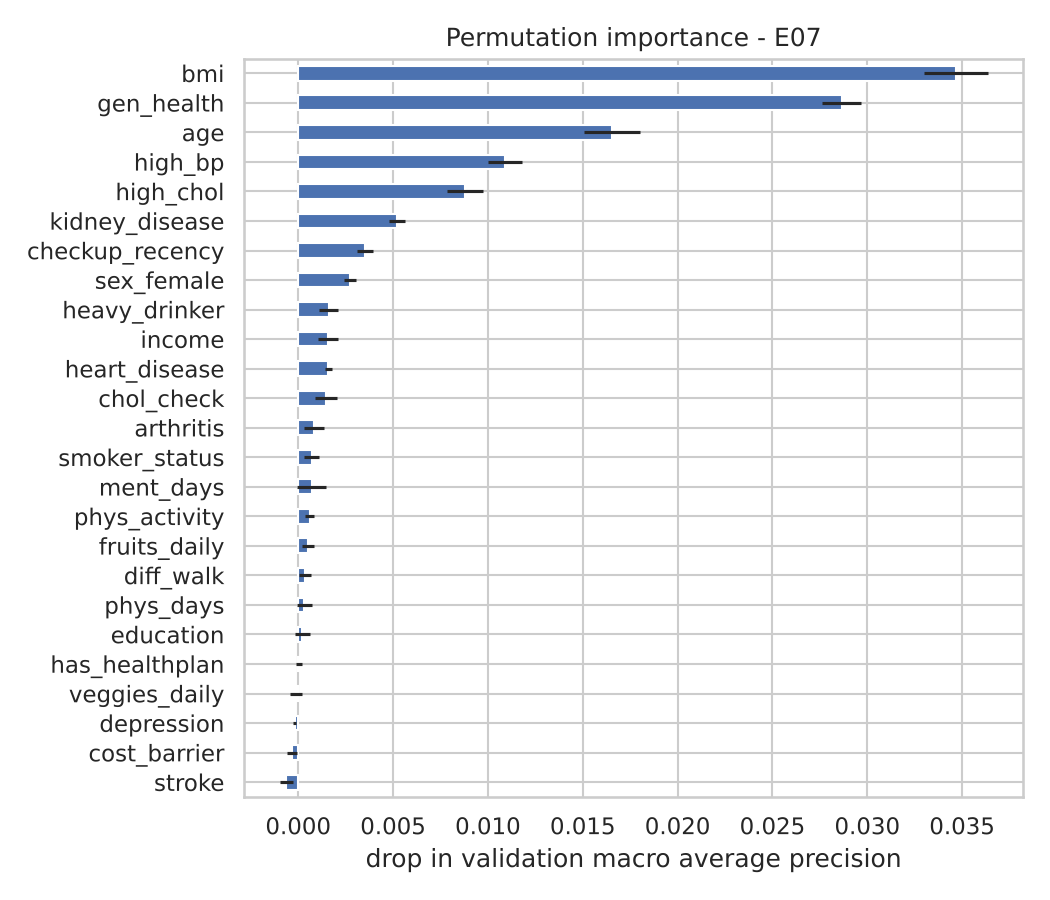
\includegraphics[width=0.48\linewidth]{fig10_permutation_importance.png}
\caption{Left: training vs.\ validation log-loss across boosting iterations for E07. Right: permutation importance (drop in validation macro AP) for E07.}
\end{figure}

\begin{figure}[H]
\centering
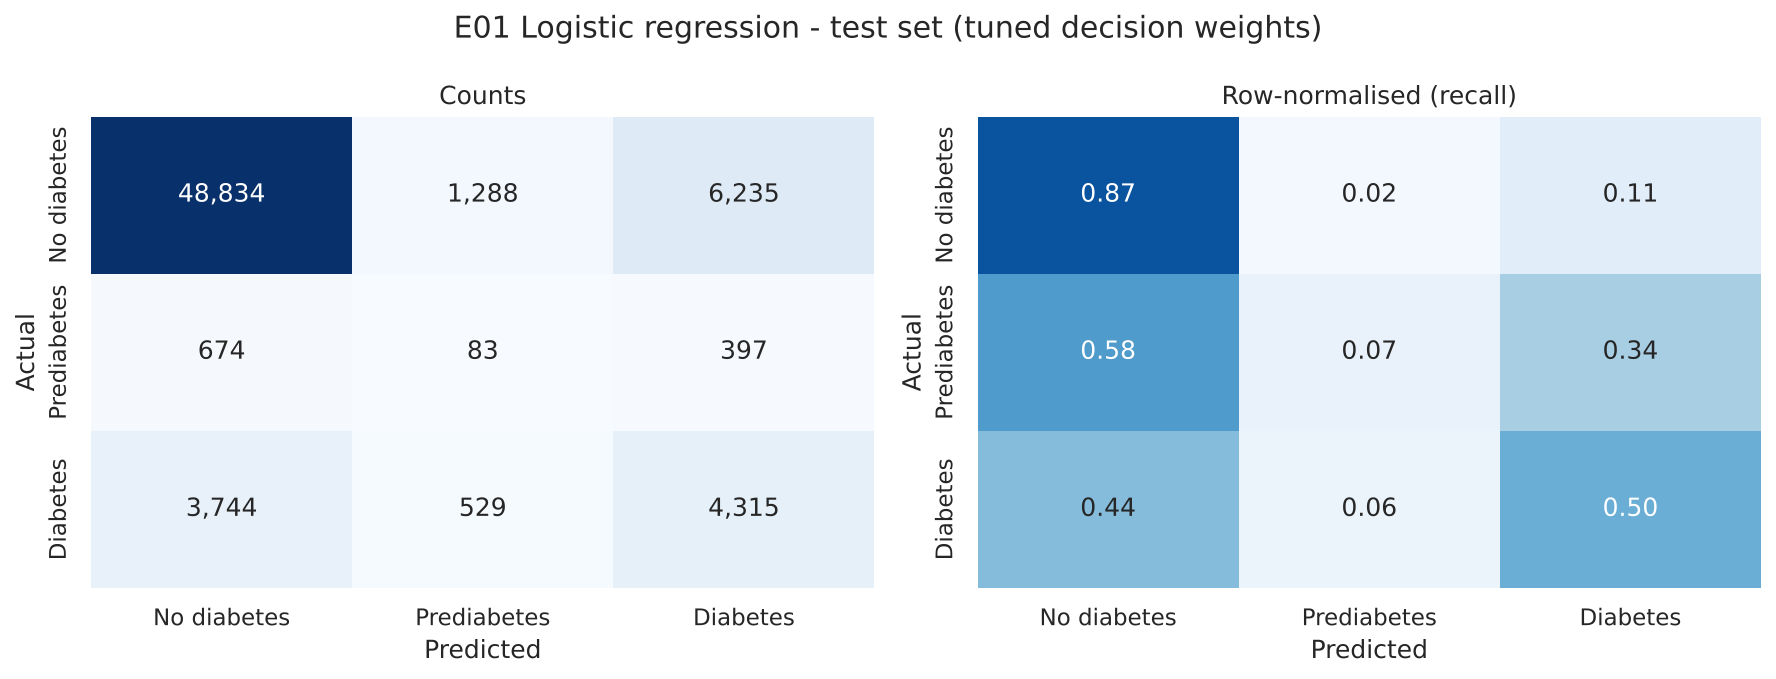
\includegraphics[width=0.49\linewidth]{fig08_confusion_E01.png}\hfill
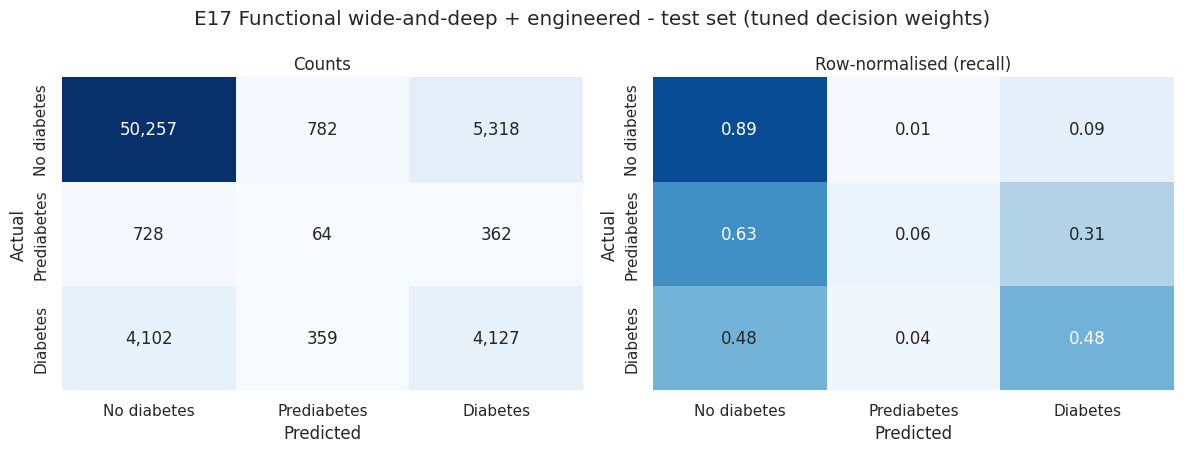
\includegraphics[width=0.49\linewidth]{fig08_confusion_E17.png}
\caption{Test-set confusion matrices for logistic regression (E01, left) and the wide-and-deep network (E17, right) with tuned decision weights.}
\end{figure}

\section{Reproducibility}
The environment (Python 3.13, scikit-learn 1.6.1, TensorFlow 2.21, Keras 3.13.2, SHAP 0.52.0) is pinned in \texttt{requirements.txt} and recorded in \texttt{reports/environment.json}. The SHA-256 of the data file used is \texttt{bfe9e629\ldots ad300b1b9}. Saved artifacts (full scikit-learn pipeline, Keras model with its preprocessor, and metadata containing decision weights and the screening threshold) were reloaded and reproduced the in-memory predictions exactly.


\end{document}
